\documentclass[12pt]{article}
\setlength\parindent{0pt}
\usepackage{fullpage}
\usepackage{graphicx}
\usepackage{amsmath}
\setlength{\parskip}{4mm}
\def\LL{\left\langle}   % left angle bracket
\def\RR{\right\rangle}  % right angle bracket
\def\LP{\left(}         % left parenthesis
\def\RP{\right)}        % right parenthesis
\def\LB{\left\{}        % left curly bracket
\def\RB{\right\}}       % right curly bracket
\def\PAR#1#2{ {{\partial #1}\over{\partial #2}} }
\def\PARTWO#1#2{ {{\partial^2 #1}\over{\partial #2}^2} }
\def\PARTWOMIX#1#2#3{ {{\partial^2 #1}\over{\partial #2 \partial #3}} }
\newcommand{\BE}{\begin{displaymath}}
\newcommand{\EE}{\end{displaymath}}
\newcommand{\BNE}{\begin{equation}}
\newcommand{\ENE}{\end{equation}}
\newcommand{\BEA}{\begin{eqnarray}}
\newcommand{\EEA}{\nonumber\end{eqnarray}}
\newcommand{\EL}{\nonumber\\}
\newcommand{\la}[1]{\label{#1}}
\newcommand{\ie}{{\em i.e.\ }}
\newcommand{\eg}{{\em e.\,g.\ }}
\newcommand{\cf}{cf.\ }
\newcommand{\etc}{etc.\ }
\newcommand{\Tr}{{\rm tr}}
\newcommand{\etal}{{\it et al.}}
\newcommand{\OL}[1]{\overline{#1}\ } % overline
\newcommand{\OLL}[1]{\overline{\overline{#1}}\ } % double overline
\newcommand{\OON}{\frac{1}{N}} % "one over N"
\newcommand{\OOX}[1]{\frac{1}{#1}} % "one over X"



\begin{document}
\Large
\centerline{\sc{Extra Credit 1: Problems}}
\normalsize
\centerline{\sc{Due Friday, May 5, to your TA's mailbox}}

{\bf Note:} You may do either this assignment or Extra Credit 2, but not both.

{\bf Note 2:} In order to get credit for these problems, you must include text describing your reasoning. All of these problems are difficult; discuss briefly what the difficulty is with each one, and 
how you overcame it. All solutions must be well-reasoned and show all steps.

You can earn up to 0.5 points on your course average per problem, for a maximum of 3.5 points.


\begin{enumerate}

\item In a rotary clothes dryer, sometimes you see a sock move as shown. As the dryer turns (counterclockwise, here), the sock sticks to the wall for a little while,
then -- at some point -- falls off of the wall and lands back on the bottom. If the radius of the dryer is $r$ and it spins at angular velocity $\omega$, find the angle
$\theta$ above the horizontal where it loses contact with the wall.

\begin{center}
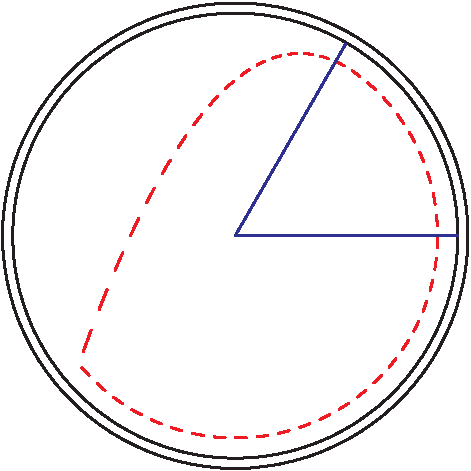
\includegraphics[width=0.5\textwidth]{sock-crop.pdf}
\end{center}

\item An untrained bowler doesn't put any spin on the ball -- he just throws the ball down the lane. Suppose that the ball (moment of inertia $\frac{2}{5}mr^2$)
begins its motion moving at speed $v$, but with $\omega_0 = 0$. Gradually, friction will make the ball start rotating.
If the coefficient of kinetic friction between the ball and the lane is $\mu_k$, how long does it take
for the ball to begin rolling without slipping?

\item Two buckets of masses $m_1$ and $m_2$ are connected to a string which hangs over a cylindrical pulley of mass $m_3$. Find the acceleration of the buckets.

\item Suppose that you attach a string to a rock and are whirling it around in a circle. (You may neglect gravity for this problem, so the only force on the rock is the tension of the string.)
Initially, the string has a length $R$ and angular velocity $\omega$.
\begin{enumerate}
\item Suppose that you shorten the string so that it is now length $R/2$. Find the new value of $\omega$.
\item By how much did the kinetic energy change in this process?
\item If the kinetic energy changed, show that this is consistent with the work-energy theorem, $\Delta KE = \int \vec F \cdot d\vec s$. (First, you will need to think about what ``force'' we are talking about here.)
\end{enumerate}

\item A certain car has a maximum engine power of 100 kW and a mass of 1000 kg. The coefficient of static friction between the tires and the pavement is 0.8. The driver of this car wants to accelerate from a stop to 
30 m/s as quickly as possible. (You may neglect air resistance.) How long does this take? (Note: I gave you both the engine power and the coefficient of friction. You need both for your answer; you will need to think about why.)

\item A jet-powered sled has a motor that takes a little while to warm up. For the first moments of its ignition, the force it exerts is $F=\beta t$, where $\beta$ is some constant. The coefficients of static and kinetic
friction between the sled and the ground are $\mu_s$ and $\mu_k$, respectively; the sled's mass is $m$. 

\begin{enumerate}
\item How long will it take for the sled to start moving?
\item Write down a (piecewise-defined, if necessary) function for the sled's position as a function of time. 
\end{enumerate}

\item A moon orbits a planet in a circular orbit at distance $r$ and angular velocity $\omega$. An engineer would like to place a satellite somewhere between the moon and the planet so that it, 
also, orbits the planet in a circular orbit with angular velocity $\omega$, synchronized with the orbit of the moon. 

Somewhere between the moon and the planet, at some intermediate radius $R$ between 0 and $R$, there is a point (called a ``Lagrange point''), where this is possible. Find $R$. 

\end{enumerate}

\newpage
\Large
\centerline{\sc{Extra Credit 2: Interpretation}}
\normalsize
\centerline{\sc{Due Friday, May 5, to your TA's mailbox}}

\normalsize

{\bf Note:} You may do either this assignment or Extra Credit 1, but not both. Each problem is worth up to 0.5 points on your final average, for a maximum of 3.5 points.

{\bf Instructions:} For each problem, write a substantial discussion answering it. You may elect to type your responses; if you do, feel free to type out equations as you
would in a graphing calculator. Your responses will involve some diagrams and perhaps some algebra depending on the problem, but this extra credit assignment is more about
{\it interpretation} and discussion, rather than the ability to solve particularly difficult problems. 

\begin{enumerate}

\item Many simple machines use the concept of ``mechanical advantage'', whereby a machine converts a small force acting over a large distance to a large force acting over a small distance. Find four problems (homework, 
recitation, or exams), or classroom demos, where this concept comes up, and discuss how the concept of mechanical advantage is related to the laws of physics and the engineering at work in the problem. Also discuss how,
even though the machine amplifies a force, energy is still conserved. Then, choose either a hydraulic lift, a car's transmission, or a bolt cutter. Draw a simplified version of the machine, and discuss how the laws of physics that we have discussed
create mechanical advantage but do not violate the conservation of energy. 

\item Looking back at your homework or exams, find four examples of problems whose solutions were simpler than you thought they were. Discuss the techniques involved in solving them and how, based on what you know now,
you would be able to look at those problems and approach them in a more straightforward, physically-correct way.

\item In a rotary clothes dryer, sometimes you see a sock move as shown. As the dryer turns (counterclockwise, here), the sock sticks to the wall for a little while,
then -- at some point -- falls off of the wall and lands back on the bottom. If the radius of the dryer is $r$ and it spins at angular velocity $\omega$, find the angle
$\theta$ above the horizontal where it loses contact with the wall. (Note that this problem appears here in addition to Extra Credit 1 because it is an example of the previous idea -- that physics is simpler than we often think! Many of the TA's worked on this problem for a while before we were able to come up with the solution, which is
deceptively simple; all that it requires is that you take the laws of physics seriously.)

\begin{center}
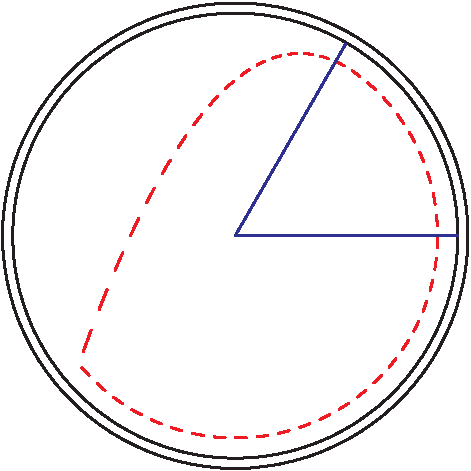
\includegraphics[width=0.5\textwidth]{sock-crop.pdf}
\end{center}

\item Write a problem that would be suitable for an exam, then solve it. Discuss why you chose to write your problem in the way that you did, and what concepts it is supposed to test. What aspects are students likely 
going to find challenging? Which of our previous exam questions might this replace?

\item When I was in the Arizona mountains camping with some friends, I drove my car (an old Saturn, a small front-wheel drive car) down a hillside covered in scree (loose rocks that don't give much traction). My car negotiated
this hill without a problem. Later that night, a large group of people came by with a SUV and a pickup truck. They had something of a party (and got a bit drunk), and then 
decided to leave. One of the pickup trucks got stuck at the bottom of the hill. When the driver tried to drive up the hill,
the rear wheels of the truck spun, and it didn't move. 

In order to try to get up the hill, they got a large member of their group to stand on the rear bumper of the truck. 
The driver again tried to accelerate, but the wheels just spun. Finally, they got the person standing on the
bumper to jump up and down while the driver pressed the accelerator. When the person on the bumper came down from a jump, the truck lurched forward. As this was happening, the guy on the bumper fell off on the ground.
The wheels of the truck then began to spin again, spraying him with loose rock as he scrambled out of the way.

Describe the physics of this process. What is going on? Why did these things happen? Why did my small car not have a problem with this?

\item Write out a solution to HW4 Problem 5, using only symbols ($m$'s, $g$, $\theta$, $\mu$'s, and so on). Then, describe the physical identification of each term that appears in your algebra, as much as possible.
For instance, if you see ``$mg \cos \theta$'', you might identify that as ``the component of weight perpendicular to the surface.''

\item Do the same for HW2 Problem 5.

\end{enumerate}

\end{document}
